\chapter{Materials and sections}
\section{Stardard uniaxial materials}
\subsection{defElasticMaterial}
\noindent Construct an elastic uniaxial material
\begin{verbatim}
defElasticMaterial(mdlr,name,E)
\end{verbatim}
\vspace{-10pt}
{\color{grayLines} \rule{\linewidth}{0.25pt}}
\begin{center}
\begin{tabular}{lp{10cm}}
{\tt mdlr} & modeler name \\
{\tt name} & name identifying the material \\
{\tt E} & tangent in the stress-strain diagram (see figure \ref{Elastic}) \\
\end{tabular}
\end{center}
\paragraph{Example}
\begin{verbatim}
*
\end{verbatim}

\begin{figure}[h]
\centering
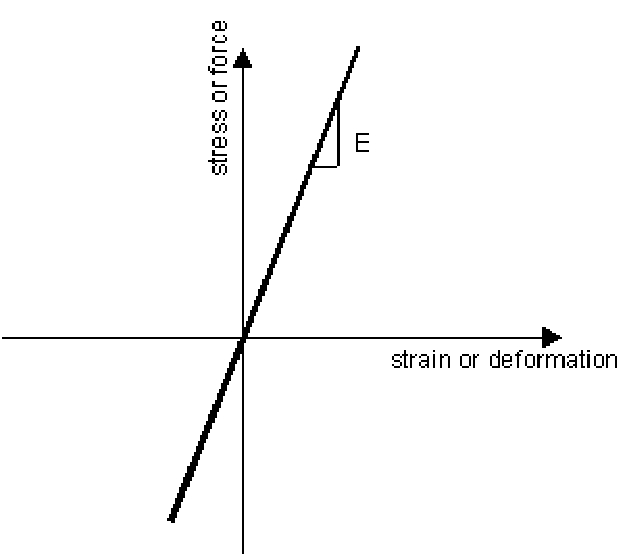
\includegraphics[width=60mm]{materials/figures/Elastic}
\caption{Elastic uniaxial material. Stress-strain diagram}\label{Elastic}
\end{figure}

\subsection{defElasticPPMaterial}
\noindent Construct an elastic perfectly-plastic uniaxial material
\begin{verbatim}
defElasticPPMaterial(mdlr,name,E,fyp,fyn)
\end{verbatim}
\vspace{-10pt}
{\color{grayLines} \rule{\linewidth}{0.25pt}}
\begin{center}
\begin{tabular}{lp{10cm}}
{\tt mdlr} & modeler name \\
{\tt name} & name identifying the material \\
{\tt E} & tangent in the elastic zone of the stress-strain diagram (see figure \ref{ElasticPP}) \\
{\tt fyp} & stress at which material reaches plastic state in tension (see figure \ref{ElasticPP}) \\
{\tt fyn} &  stress at which material reaches plastic state in compression (see figure \ref{ElasticPP}) \\
{\tt } &  \\
\end{tabular}
\end{center}
\paragraph{Example}
\begin{verbatim}
*
\end{verbatim}

\begin{figure}[h]
\centering
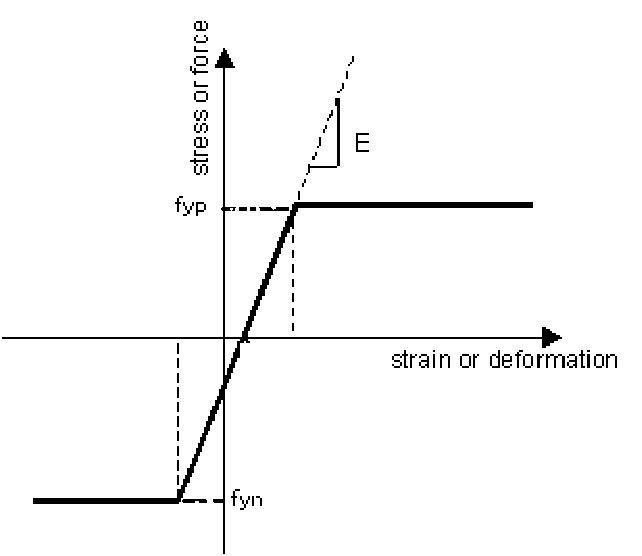
\includegraphics[width=60mm]{materials/figures/ElasticPP}
\caption{Elastic perfectly-plastic uniaxial material. Stress-strain diagram}\label{ElasticPP}
\end{figure}

\subsection{defElastNoTracMaterial}
\noindent Construct a uniaxial elastic-no tension material
\begin{verbatim}
defElastNoTracMaterial(mdlr,name,E)
\end{verbatim}
\vspace{-10pt}
{\color{grayLines} \rule{\linewidth}{0.25pt}}
\begin{center}
\begin{tabular}{lp{10cm}}
{\tt mdlr} & modeler name \\
{\tt name} & name identifying the material \\
{\tt E} & tangent in the elastic zone of the stress-strain diagram (see figure \ref{ENT}) \\
\end{tabular}
\end{center}
\paragraph{Example}
\begin{verbatim}
*
\end{verbatim}
\begin{figure}[h]
\centering
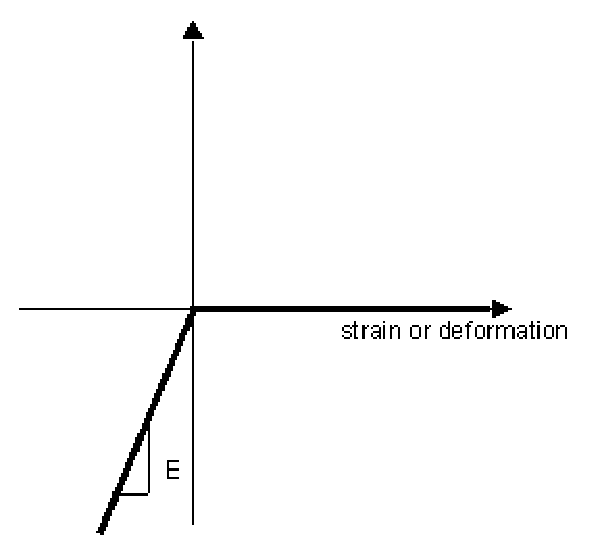
\includegraphics[width=50mm]{materials/figures/ENT}
\caption{Elastic-no tension material. Stress-strain diagram}\label{ENT}
\end{figure}

\section{Steel and reinforcing steel materials}
\subsection{defCableMaterial}
\noindent Construct a uniaxial bilinear prestressed material. The stress strain ranges from slack (large strain at zero stress) to taught (linear with modulus E).
\begin{verbatim}
defCableMaterial(mdlr,name,E,prestress,rho)
\end{verbatim}
\vspace{-10pt}
{\color{grayLines} \rule{\linewidth}{0.25pt}}
\begin{center}
\begin{tabular}{lp{10cm}}
{\tt mdlr} & modeler name \\
{\tt name} & name identifying the material \\
{\tt E} & Young modulus \\
{\tt prestress} & prestress \\
{\tt rho} & effective self weight (gravity component of weight per volume transverse to the cable) \\
\end{tabular}
\end{center}
\paragraph{Example}
\begin{verbatim}
*
\end{verbatim}


\subsection{defSteel01}
\noindent Construct a uniaxial bilinear steel material object with kinematic hardening
\begin{verbatim}
defSteel01(mdlr,name,E,fy,b)
\end{verbatim}
\vspace{-10pt}
{\color{grayLines} \rule{\linewidth}{0.25pt}}
\begin{center}
\begin{tabular}{lp{10cm}}
{\tt mdlr} & modeler name \\
{\tt name} & name identifying the material \\
{\tt E} & initial elastic tangent (see figure \ref{Steel01}) \\
{\tt fy} &  yield strength (see figure \ref{Steel01})\\
{\tt b} &  strain-hardening ratio: ratio between post-yield tangent and initial elastic tangent (see figure \ref{Steel01})\\
\end{tabular}
\end{center}
\paragraph{Example}
\begin{verbatim}
*
\end{verbatim}

\begin{figure}[h]
\centering
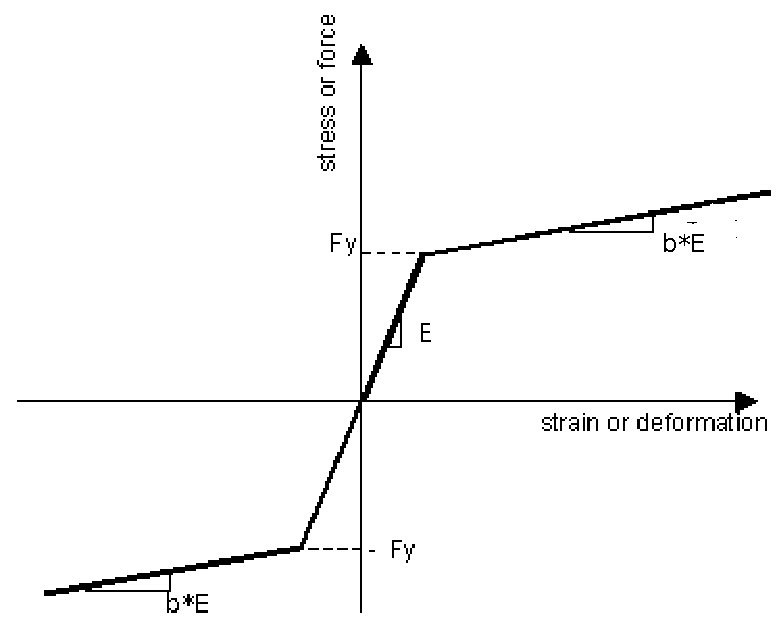
\includegraphics[width=60mm]{materials/figures/Steel01}
\caption{Steel001: uniaxial bilinear steel material with kinematic hardening. Stress-strain diagram}\label{Steel01}
\end{figure}


\subsection{defSteel02}
\noindent Construct a uniaxial Giuffre-Menegotto-Pinto steel material object with isotropic strain hardening
\begin{verbatim}
defSteel02(mdlr,name,E,fy,b,initialStress)
\end{verbatim}
\vspace{-10pt}
{\color{grayLines} \rule{\linewidth}{0.25pt}}
\begin{center}
\begin{tabular}{lp{10cm}}
{\tt mdlr} & modeler name \\
{\tt name} & name identifying the material \\
{\tt E} & initial elastic tangent (see figure \ref{Steel02}) \\
{\tt fy} &  yield strength (see figure \ref{Steel02})\\
{\tt b} &  strain-hardening ratio: ratio between post-yield tangent and initial elastic tangent)\\
{\tt initialStress} &  initial stress \\
\end{tabular}
\end{center}
{\footnotesize The transition from elastic to plastic branches  (see figure \ref{Steel02}) is controlled by parameters R0, R1, R2. The default values R0=15, R1=0.925 and R2=0.15}
\paragraph{Example}
\begin{verbatim}
*
\end{verbatim}

\begin{figure}[h]
\centering
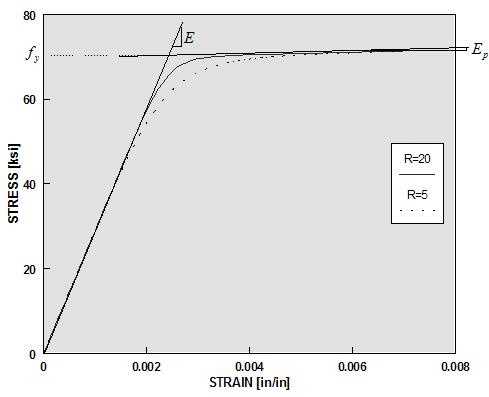
\includegraphics[width=60mm]{materials/figures/Steel02Monotonic}
\caption{Steel002: uniaxial bilinear steel material with isotropic strain hardening. Stress-strain diagram}\label{Steel02}
\end{figure}

\subsection{ReinforcingSteel}
\noindent This class constructs a bilinear stress-strain diagram to carry out the analysis of reinforced concrete according to Eurocode 2. Other national standards, like the spanish EHE and the swiss SIA also adopt this diagram.

\begin{center}
\begin{tabular}{lp{10cm}}
\multicolumn{2}{p{11cm}}{\color{grayText} \large{Parameters}} \\
\multicolumn{2}{p{13cm}}{\color{grayLines} \rule{\linewidth}{0.25pt}} \\
{\tt nmbMaterial} & name identifying the material \\
{\tt nmbDiagK} & name identifying the characteristic stress-strain diagram (default: {\tt "dgK"+nmbMaterial}) \\
{\tt tagDiagK} & tag of the uniaxial material with the characteristic stress-strain diagram\\
{\tt nmbDiagD} &  name identifying the design stress-strain diagram (default: {\tt "dgD"+nmbMaterial}) \\
{\tt tagDiagD} & tag of the uniaxial material with the design stress-strain diagram\\
{\tt fyk} & characteristic value of the yield strength\\
{\tt gammaS} & partial factor for material (default: 1.15)\\
{\tt Es} & elastic modulus of the material (default: 2e11)\\
{\tt emax} & maximum strain at failure point\\
{\tt k} & ratio between characteristic ultimate stress and characteristic yield stress $^{(1)}$ (default: 1.05)\\
\multicolumn{2}{p{13cm}}{\color{grayLines} \rule{\linewidth}{0.25pt}} \\
\multicolumn{2}{p{13cm}}{\footnotesize{(1): according to annex C of EC2: for class A k$\ge$1,05, for class B k$\ge$1,08}}
\end{tabular}
\end{center}

\begin{center}
\begin{tabular}{lp{9cm}}
\multicolumn{2}{p{11cm}}{\color{grayText} \large{Methods}} \\
\multicolumn{2}{p{13cm}}{\color{grayLines} \rule{\linewidth}{0.25pt}} \\
{\tt fmaxk()} & characteristic ultimate strength \\
{\tt fyd()} & design yield stress \\
{\tt eyk()} & characteristic strain at yield point\\
{\tt eyd()} & design strain at yield point\\
{\tt Esh()} &  post-yield tangent\\
{\tt bsh()} & ratio between post-yield tangent and initial elastic tangent\\
{\tt defDiagK(mdlr)} & returns XC uniaxial material (characteristic values)\\
{\tt defDiagD(mdlr)} & returns XC uniaxial material (design values)\\
\end{tabular}
\end{center}

\section{Concrete materials}
\subsection{defConcrete01}
\noindent Construct a uniaxial Kent-Scott-Park concrete material object with degraded linear unloading/reloading stiffness according to the work of Karsan-Jirsa and no tensile strength.
\begin{verbatim}
defConcrete01(mdlr,name,epsc0,fpc,fpcu,epscu)
\end{verbatim}
\vspace{-10pt}
{\color{grayLines} \rule{\linewidth}{0.25pt}}
\begin{center}
\begin{tabular}{lp{10cm}}
{\tt mdlr} & modeler name \\
{\tt name} & name identifying the material \\
{\tt fpc} &  concrete compressive strength at 28 days (compression is negative) $^{(1)}$\\
{\tt epsc0} &  concrete strain at maximum strength (see figure \ref{Concrete01}) $^{(2)}$\\
{\tt fpcu} &  concrete crushing strength (see figure \ref{Concrete01}) \\
{\tt epscu} &  concrete strain at crushing strength (see figure \ref{Concrete01}) \\
\hline
\multicolumn{2}{p{12cm}}{\footnotesize(1): Compressive concrete parameters should be input as negative values (if input as positive, they will be converted to negative internally)}\\
\multicolumn{2}{p{12cm}}{\footnotesize (2): The initial slope for this model is $2*fpc/epsc0$ (see figure \ref{Concrete01})}\\
\end{tabular}
\end{center}
\paragraph{Example}
\begin{verbatim}
*
\end{verbatim}

\begin{figure}[h]
\centering
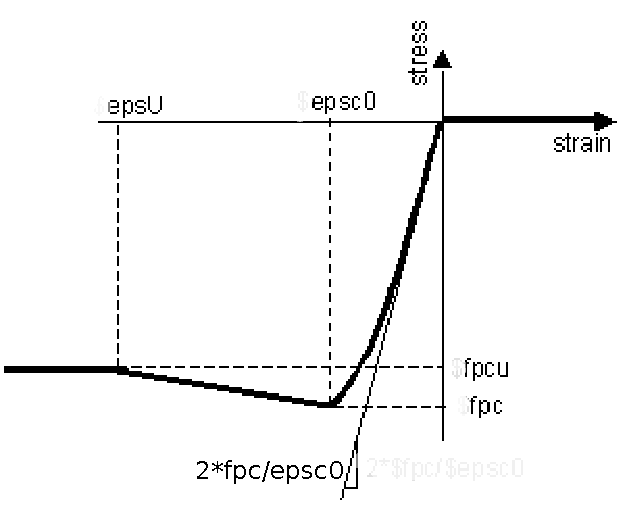
\includegraphics[width=60mm]{materials/figures/Concrete01}
\caption{Concrete01: uniaxial Kent-Scott-Park concrete material. Stress-strain diagram}\label{Concrete01}
\end{figure}

\section{ND materials}
An ND material is an object that represents the stress-strain relationship at the gauss-point of a continuum element.

\subsection{defElasticIsotropic3d}
\noindent Construct an elastic isotropic material.
\begin{verbatim}
defElasticIsotropic3d(mdlr,name,E,nu,rho)
\end{verbatim}
\vspace{-10pt}
{\color{grayLines} \rule{\linewidth}{0.25pt}}
\begin{center}
\begin{tabular}{lp{10cm}}
{\tt mdlr} & modeler name \\
{\tt name} & name identifying the material\\
{\tt E} & elastic modulus \\
{\tt nu} & Poisson's ratio \\
{\tt rho} &  mass density, optional (default = 0.0)\\
\end{tabular}
\end{center}
\paragraph{Example}
\begin{verbatim}
*
\end{verbatim}

\subsection{defElasticIsotropicPlaneStrain}
\noindent Construct an elastic isotropic plane-strain material.
\begin{verbatim}
defElasticIsotropicPlaneStrain(mdlr,name,E,nu,rho)
\end{verbatim}
\vspace{-10pt}
{\color{grayLines} \rule{\linewidth}{0.25pt}}
\begin{center}
\begin{tabular}{lp{10cm}}
{\tt mdlr} & modeler name \\
{\tt name} & name identifying the material\\
{\tt E} & elastic modulus \\
{\tt nu} & Poisson's ratio \\
{\tt rho} &  mass density, optional (default = 0.0)\\
\end{tabular}
\end{center}
\paragraph{Example}
\begin{verbatim}
*
\end{verbatim}

\subsection{defElasticIsotropicPlaneStress}
\noindent Construct an elastic isotropic plane-stress material.
\begin{verbatim}
defElasticIsotropicPlaneStress(mdlr,name,E,nu,rho)
\end{verbatim}
\vspace{-10pt}
{\color{grayLines} \rule{\linewidth}{0.25pt}}
\begin{center}
\begin{tabular}{lp{10cm}}
{\tt mdlr} & modeler name \\
{\tt name} & name identifying the material\\
{\tt E} & elastic modulus \\
{\tt nu} & Poisson's ratio \\
{\tt rho} &  mass density, optional (default = 0.0)\\
\end{tabular}
\end{center}
\paragraph{Example}
\begin{verbatim}
*
\end{verbatim}
\section{Sections}
A section represents a force-deformation (or resultant stress-strain) relationship at beam-column or plate element.

Three types of sections are going to be considered:
\begin{description}
\item{Elastic:} defined by material and geometric constants;
\item{Resultant:} general nonlinear description of force-deformation response, e.g. moment-curvature;
\item{Fiber:} section is discretized into smaller regions for which the material stress-strain response is integrated to give resultant behavior, e.g. reinforced concrete.
\end{description}
\subsection{Elastic sections}
\subsubsection{defElasticSection2d}
\noindent Construct an elastic section appropiate for 2D beam analysis.
\begin{verbatim}
defElasticSection2d(mdlr,name,A,E,I)
\end{verbatim}
\vspace{-10pt}
{\color{grayLines} \rule{\linewidth}{0.25pt}}
\begin{center}
\begin{tabular}{lp{10cm}}
{\tt mdlr} & modeler name \\
{\tt name} & name identifying the section \\
{\tt A} &  cross-sectional area of the section \\
{\tt E} &  Young's modulus of material \\
{\tt I} &  second moment of area about the local z-axis\\
\end{tabular}
\end{center}
\paragraph{Example}
\begin{verbatim}
*
\end{verbatim}


\subsubsection{defElasticShearSection2d}
\noindent Construct an elastic section appropiate for 2D beam analysis, including shear deformations.
\begin{verbatim}
defElasticShearSection2d(mdlr,name,A,E,G,I,alpha)
\end{verbatim}
\vspace{-10pt}
{\color{grayLines} \rule{\linewidth}{0.25pt}}
\begin{center}
\begin{tabular}{lp{10cm}}
{\tt mdlr} & modeler name \\
{\tt name} & name identifying the section \\
{\tt A} &  cross-sectional area of the section \\
{\tt E} &  Young's modulus of material \\
{\tt G} & shear modulus \\
{\tt I} &  second moment of area about the local z-axis\\
{\tt alpha} & shear shape factor \\
\end{tabular}
\end{center}
\paragraph{Example}
\begin{verbatim}
*
\end{verbatim}

\subsubsection{defElasticSectionFromMechProp2d}
\noindent Construct an elastic section appropiate for 2D beam analysis, taking mechanical properties of the section form a MechProp2d object.
\begin{verbatim}
defElasticSectionFromMechProp2d(mdlr,name,mechProp2d)
\end{verbatim}
\vspace{-10pt}
{\color{grayLines} \rule{\linewidth}{0.25pt}}
\begin{center}
\begin{tabular}{lp{10cm}}
{\tt mdlr} & modeler name \\
{\tt name} & name identifying the section \\
{\tt mechProp2d} & object that contains mechanical properties of the section  \\
\end{tabular}
\end{center}
\paragraph{Example}
\begin{verbatim}
*
\end{verbatim}

%%%
\subsubsection{defElasticSection3d}
\noindent Construct an elastic section appropiate for 3D beam analysis.
\begin{verbatim}
defElasticSection3d(mdlr,name,A,E,G,Iz,Iy,J)
\end{verbatim}
\vspace{-10pt}
{\color{grayLines} \rule{\linewidth}{0.25pt}}
\begin{center}
\begin{tabular}{lp{10cm}}
{\tt mdlr} & modeler name \\
{\tt name} & name identifying the section \\
{\tt A} &  cross-sectional area of the section \\
{\tt E} &  Young's modulus of material \\
{\tt Iz} &  second moment of area about the local z-axis\\
{\tt Iy} &  second moment of area about the local y-axis\\
{\tt J} & torsional moment of inertia of the section \\
\end{tabular}
\end{center}
\paragraph{Example}
\begin{verbatim}
*
\end{verbatim}


\subsubsection{defElasticShearSection3d}
\noindent Construct an elastic section appropiate for 3D beam analysis, including shear deformations.
\begin{verbatim}
defElasticShearSection3d(mdlr,name,A,E,G,Iz,Iy,J,alpha)
\end{verbatim}
\vspace{-10pt}
{\color{grayLines} \rule{\linewidth}{0.25pt}}
\begin{center}
\begin{tabular}{lp{10cm}}
{\tt mdlr} & modeler name \\
{\tt name} & name identifying the section \\
{\tt A} &  cross-sectional area of the section \\
{\tt E} &  Young's modulus of material \\
{\tt G} & shear modulus \\
{\tt Iz} &  second moment of area about the local z-axis\\
{\tt Iy} &  second moment of area about the local y-axis\\
{\tt J} & torsional moment of inertia of the section \\
{\tt alpha} & shear shape factor \\
\end{tabular}
\end{center}
\paragraph{Example}
\begin{verbatim}
*
\end{verbatim}

\subsubsection{defElasticSectionFromMechProp3d}
\noindent Construct an elastic section appropiate for 3D beam analysis, taking mechanical properties of the section form a MechProp3d object.
\begin{verbatim}
defElasticSectionFromMechProp3d(mdlr,name,mechProp3d)
\end{verbatim}
\vspace{-10pt}
{\color{grayLines} \rule{\linewidth}{0.25pt}}
\begin{center}
\begin{tabular}{lp{10cm}}
{\tt mdlr} & modeler name \\
{\tt name} & name identifying the section \\
{\tt mechProp3d} & object that contains mechanical properties of the section  \\
\end{tabular}
\end{center}
\paragraph{Example}
\begin{verbatim}
*
\end{verbatim}

\subsubsection{defElasticMembranePlateSection}
\noindent Construct an an isotropic elastic section appropriate for plate and shell analysis.
\begin{verbatim}
defElasticMembranePlateSection(mdlr,name,E,nu,rho,h)
\end{verbatim}
\vspace{-10pt}
{\color{grayLines} \rule{\linewidth}{0.25pt}}
\begin{center}
\begin{tabular}{lp{10cm}}
{\tt mdlr} & modeler name \\
{\tt name} & name identifying the section\\
{\tt E} &  Young's modulus\\
{\tt nu} &  Poisson's modulus\\
{\tt rho} &  mass density\\
{\tt h} &  depth of section\\
\end{tabular}
\end{center}
\paragraph{Example}
\begin{verbatim}
*
\end{verbatim}

\subsubsection{defElasticPlateSection}
\noindent Construct an an isotropic elastic section appropriate for plate analysis.
\begin{verbatim}
defElasticPlateSection(mdlr,name,E,nu,rho,h)
\end{verbatim}
\vspace{-10pt}
{\color{grayLines} \rule{\linewidth}{0.25pt}}
\begin{center}
\begin{tabular}{lp{10cm}}
{\tt mdlr} & modeler name \\
{\tt name} & name identifying the section\\
{\tt E} &  Young's modulus\\
{\tt nu} &  Poisson's modulus\\
{\tt rho} &  mass density\\
{\tt h} &  depth of section\\
\end{tabular}
\end{center}
\paragraph{Example}
\begin{verbatim}
*
\end{verbatim}

\sbusection{Fiber sections}

\end{document}




\subsection{}
\noindent 
\begin{verbatim}

\end{verbatim}
\vspace{-10pt}
{\color{grayLines} \rule{\linewidth}{0.25pt}}
\begin{center}
\begin{tabular}{lp{10cm}}
{\tt mdlr} & modeler name \\
{\tt name} & name identifying the \\
{\tt } &  \\
{\tt } &  \\
{\tt } &  \\
\end{tabular}
\end{center}
\paragraph{Example}
\begin{verbatim}
*
\end{verbatim}

\begin{figure}[h]
\centering
\includegraphics[width=60mm]{materials/figures/}
\caption{. Stress-strain diagram}\label{}
\end{figure}
